\chapter{Implementasi dan Pengujian}
\label{chap: implemenPengujian}

Pada bagian ini merupakan rincian atau penjelasan lanjut mengenai lingkungan implementasi perangkat keras maupun perangkat lunak sistem informasi penilaian sidang skripsi 2. Bagian terakhir akan membahas tentang pengujian yang telah dilakukan pada sistem informasi.

\section{Implementasi}
\label{sec: implementasi}

	Pada bagian ini akan dijabarkan lingkungan pengembangan sistem informasi dan pengujian.
	
	\subsection{Lingkungan Implementasi dan Pengujian}
	\label{sub: lingkunganImp}
	
	Impelementasi dilakukan dengan menggunakan sebuah laptop. Berikut adalah spesifikasi laptop
	yang digunakan:
	
	\begin{enumerate}
		\item Processor: Intel(R) Core(TM) i5-3230M CPU @ 2.60GHz (4CPUs),~2.6GHz
		\item RAM : 4096 MB
		\item Sistem operasi : Windows 7 Ultimate 64-bit (6.1, Build 7601)
		\item Versi AngularJS : Version 1.5.2
		\item Versi Codeigniter : Version 3.1.3
		\item Versi TwitterBootstrap : Version 2.3.2
		\item Versi Google Chrome : Version 55.0.2883.87 m(64-bit)
	\end{enumerate}

	\subsection{Hasil Implementasi}
	\label{sub: hasilImplemen}
	
	Hasil implementasi dari penelitian ini adalah sebuah sistem informasi berbasis web yang menggunakan \textit{codeigniter}, \textit{AngularJS}, dan \textit{Twitter Bootstrap} sebagai dasar pembuatan. Aplikasi dapat diakses melalui jaringan \textit{global} dengan URL " http://sipskripsi.com ". Sistem informasi terdiri dari bagian-bagian sebagai berikut:
	
	\begin{enumerate}
		\item Bagian formulir berita acara sidang skripsi\\
		Bagian ini adalah halaman yang bersangkutan dalam pengisian data diri mahasiswa yang bersangkutan, sekaligus sebagai halaman akhir yang menyimpulkan perhitungan nilai akhir mahasiswa. Kolom penilaian pada halaman ini tidak dapat diisi secara manual kecuali kolom penilaian milik koordinator skripsi. Kolom penilaian yang lain didapatkan berdasarkan perhitungan nilai akhir masing-masing penguji.
		\begin{figure}[H]
			\centering
			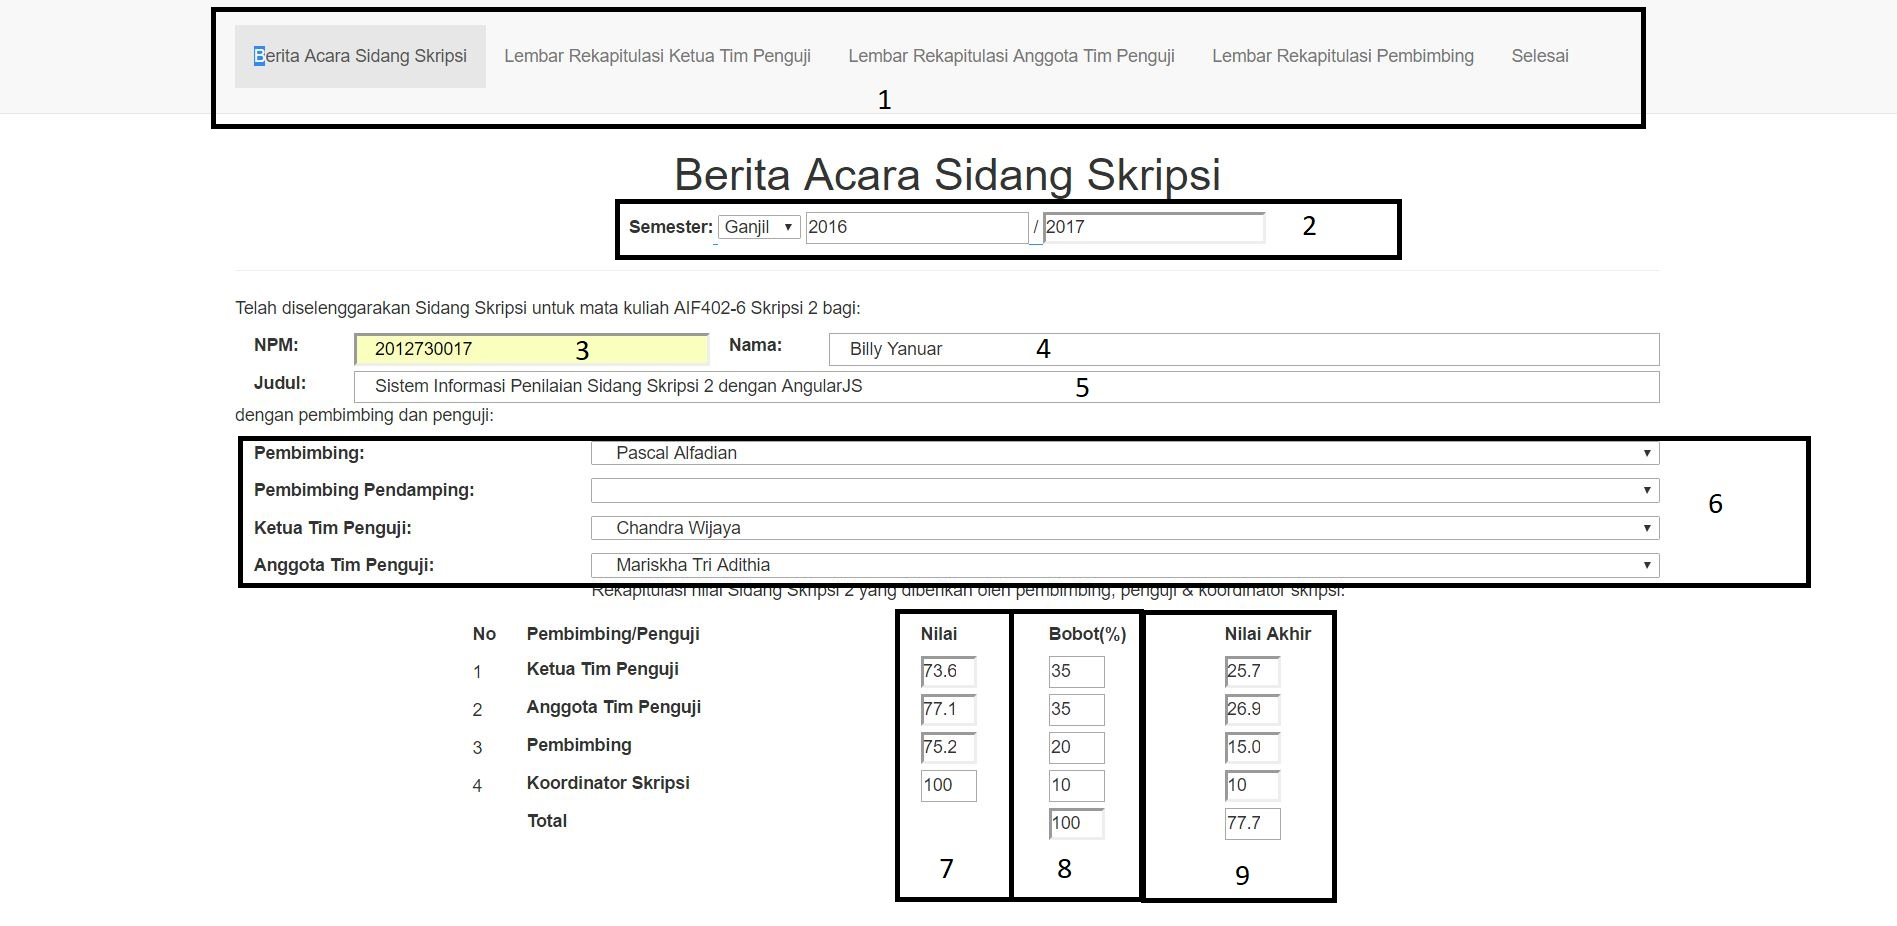
\includegraphics[scale=0.5]{Gambar/beritaacaraisi}
			\caption{Formulir berita acara sidang skripsi 2 terisi}
			\label{fig:beritaisi}
		\end{figure}
		\item Bagian formulir rekapitulasi penilaian sidang skripsi 2.\\
		Bagian ini adalah halaman yang bersangkutan dalam menampung nilai-nilai yang diberikan oleh ketua tim penguji, anggota tim penguji, dan pembimbing pada mahasiswa. 
		\begin{figure}[H]
			\centering
			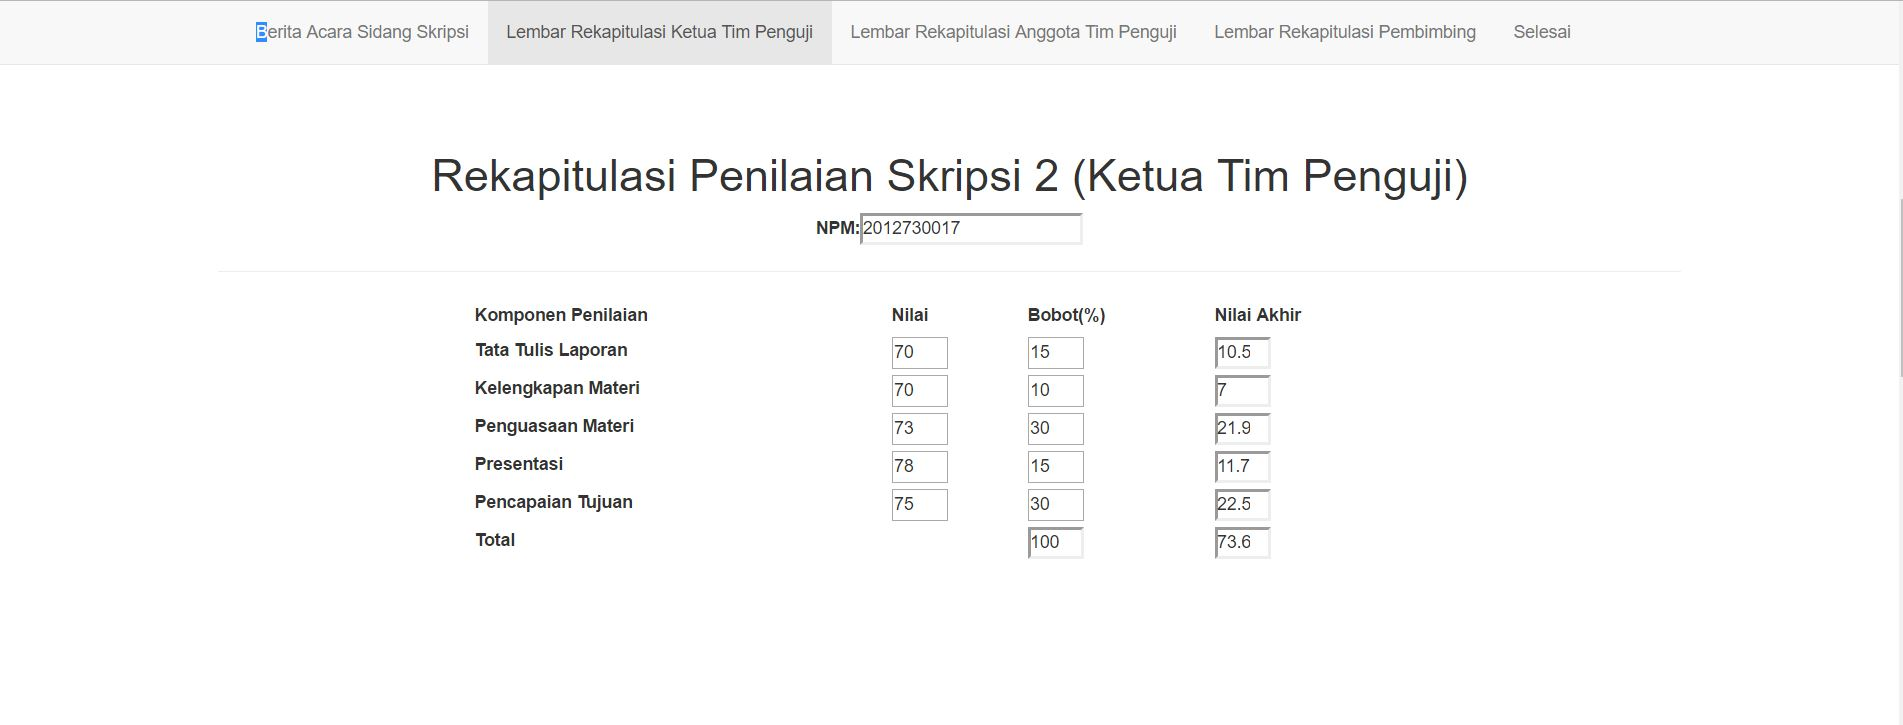
\includegraphics[scale=0.5]{Gambar/ketuaisi}
			\caption{Formulir rekapitulasi ketua tim penguji terisi}
			\label{fig:ketuaisi}
		\end{figure}
		\begin{figure}[H]
			\centering
			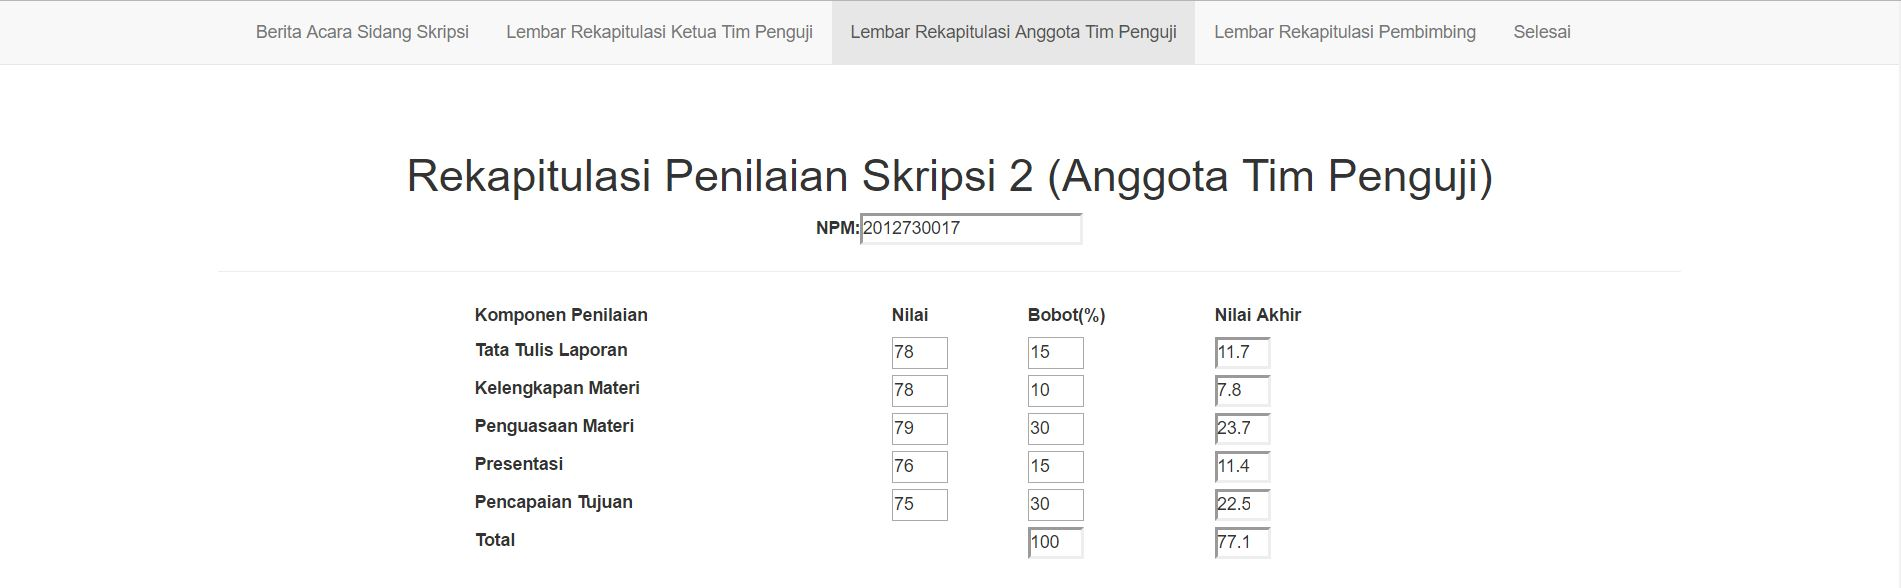
\includegraphics[scale=0.5]{Gambar/anggotaisi}
			\caption{Formulir rekapitulasi anggota tim penguji terisi}
			\label{fig:anggotaisi}
		\end{figure}
		\begin{figure}[H]
			\centering
			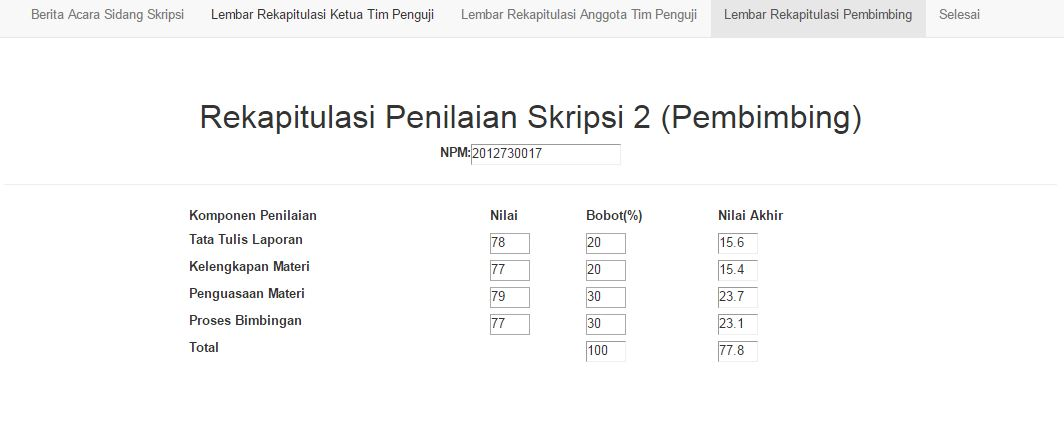
\includegraphics[scale=0.5]{Gambar/pembimbingisi}
			\caption{Formulir rekapitulasi pembimbing terisi}
			\label{fig:pembimbingisi}
		\end{figure}
		\item Bagian selesai.\\
		Bagian ini adalah bagian terakhir dari sistem informasi. Ketika formulir sudah selesai diisi, maka dengan menekan tombol selesai pada bagian ini, \textit{data} yang telah terisi akan dimasukkan ke dalam \textit{database}.
		\begin{figure}[H]
			\centering
			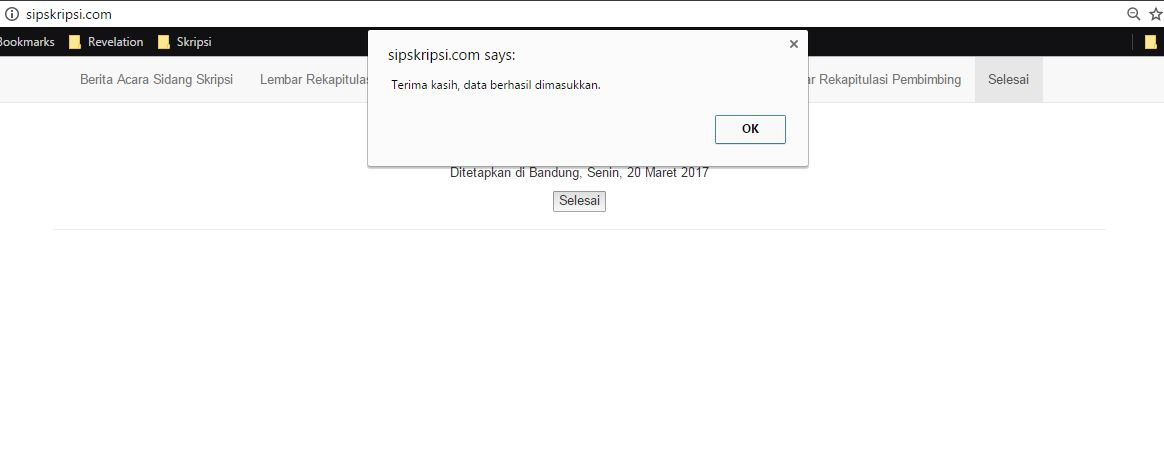
\includegraphics[scale=0.4]{Gambar/selesaiisi}
			\caption{Ketika tombol selesai di klik}
			\label{fig:selesaiisi}
		\end{figure}
		\begin{figure}[H]
			\centering
			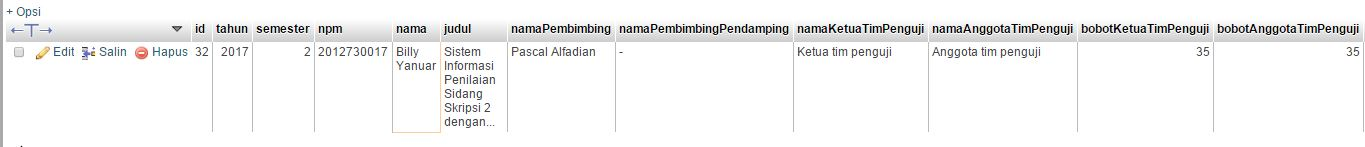
\includegraphics[scale=0.4]{Gambar/hasildatabase}
			\caption{Sebagian hasil pada database}
			\label{fig:hasildatabase}
		\end{figure}
	\end{enumerate}
	
\section{Hasil Pengujian}
\label{sec:hasilUji}

	Pengujian pada sistem informasi penilaian sidang skripsi 2 merupakan pengujian bersifat fungsional, dan pengujian eksperimental. Berikut penjelasannya:
	
	\subsection{Pengujian Eksperimental}
	\label{sub: PEksperimen}
	
	Pengujian eksperimental dilakukan dengan cara mengikuti sidang skripsi 2 yang dilakukan pada semester ganjil 2016/2017. Pada sidang yang diujikan, penilaian dilakukan dengan dua cara, yaitu dengan sistem kini yang bekerja secara manual dan dengan sistem usulan menggunakan laptop. Sehubungan dengan sifat kerasahasiaan \textit{data} pengujian, maka dengan persetujuan pembimbing pengujian eksperimental dilakukan dengan merahasiakan identitas mahasiswa yang berhubungan.
	
	Pada saat melakukan pengujian eksperimental, sistem kini memiliki kekurangan kecerobohan manusia yang mengakibatkan kesalahan dalam perhitungan nilai baik dari lembar rekapitulasi maupun lembar berita acara sidang skripsi. Hal tersebut diketahui pada saat membandingkan nilai perhitungan nilai akhir yang didapatkan oleh mahasiswa pada sistem kini dan sistem usulan. Pada beberapa kesalahan tersebut, penguji kembali melakukan perhitungan secara manual dengan menggunakan mesin hitung berupa kalkulator pada \textit{gadget} penguji. Setelah perhitungan dilakukan, didapatkan bahwa sistem usulan memiliki hasil yang benar.
	
	Percobaan eksperimental menghasilkan kesimpulan sistem usulan dapat menutupi kekurangan sistem kini yang berfokus pada perhitungan penilaian mahasiswa. Dengan menggunakan sistem usulan, perhitungan nilai dibuktikan lebih akurat dibandingkan dengan sistem kini. Berikut ini adalah salah satu hasil dari pengujian eksperimental:
	\begin{table}[htbp]
		\centering
		\caption{Tabel Pengujian Eksperimental}
		\begin{tabular}{| m{7cm} | m{5cm} |}
			\hline
			Jenis Data & Input Nilai\\
			\hline
			id & 30\\
			\hline
			tahun & 2016\\
			\hline
			semester & 1\\
			\hline
			npm & 2012730004\\
			\hline
			nama & E\\
			\hline
			judul & Watermarking\\
			\hline
			namaPembimbing & Mariskha A\\
			\hline
			namaPembimbingPendamping & -\\
			\hline
			namaKetuaTimPenguji & Husnul\\
			\hline
			namaAnggotaTimPenguji & Chandra\\
			\hline
			bobotKetuaTimPenguji & 35\\
			\hline
			bobotAnggotaTimPenguji & 35\\
			\hline
			bobotPembimbing & 20\\
			\hline
			nilaiKoordinatorSkripsi & 100\\
			\hline
			bobotKoordinatorSkripsi & 10\\
			\hline
			bobotTataTulisLaporanAnggota & 15\\
			\hline
			bobotKelengkapanMateriAnggota & 10\\
			\hline
			bobotPenguasaanMateriAnggota & 30\\
			\hline
			bobotPresentasiAnggota & 15\\
			\hline
			bobotPencapaianTujuanKetua & 30\\
			\hline
			bobotTataTulisLaporanKetua & 15\\
			\hline
			bobotKelengkapanMateriKetua & 10\\
			\hline
			bobotPenguasaanMateriKetua & 30\\
			\hline
			bobotPresentasiKetua & 15\\
			\hline
			bobotPencapaianTujuanKetua & 30\\
			\hline
			bobotTataTulisLaporanPembimbing & 20\\
			\hline
			bobotKelengkapanMateriPembimbing &20\\
			\hline
			bobotPenguasaanMateriPembimbing & 30\\
			\hline
			prosesBimbinganPembimbing & 30\\
			\hline
			nilaiAkhirMahasiswa & 84\\
			\hline
		\end{tabular}
	\end{table}
		
		
		\subsection{Pengujian Fungsional}
		\label{sub: PFungsional}
		Pengujian fungsional dilakukan untuk mengetahui apakah sistem informasi dapat menjalankan seluruh fungsi-fungsi yang dimiliki dengan baik. Hasil pengujian fungsional sistem informasi akan dijabarkan pada tabel berikut:\\
		
	\begin{table}[htbp]
		\centering
		\caption{Tabel Pengujian Fungsional}
		\begin{tabular}{| m{0.75cm} | m{7cm} | m{5cm} | m{3cm} |}
			\hline
			No & Aksi Pengguna & Reaksi yang diharapkan & Keterangan \\
			\hline
			1 & Pengguna menjalankan sistem informasi & Halaman berita acara ditampilkan & Reaksi sesuai \\
			\hline
			2 & Pengguna memasukkan nilai & Menampilkan hasil dari perhitungan otomatis & Reaksi sesuai \\
			\hline
			3 & Pengguna menekan tombol selesai & Menampilkan notifikasi data telah tersimpan & Reaksi sesuai \\
			\hline
			4 & Pengguna menekan tombol ok pada notifikasi & Menampilkan kembali halaman lembar formulir berita acara awal sebelum terisi & Reaksi sesuai \\
			\hline
		\end{tabular}
	\end{table}